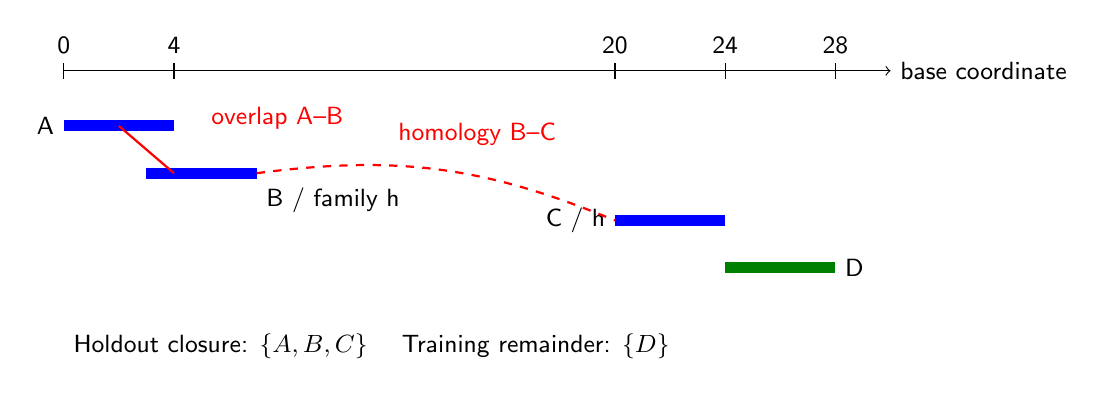
\begin{tikzpicture}[x=.35cm,y=1cm,font=\small\sffamily]
\draw[->] (0,3.7)--(30,3.7) node[right] {base coordinate};
\foreach \x in {0,4,20,24,28} {\draw (\x,3.6)--(\x,3.8);\node[above] at (\x,3.8) {\x};}
\draw[Blue,line width=4pt] (0,3)--(4,3);\node[left] at (0,3) {A};
\draw[Blue,line width=4pt] (3,2.4)--(7,2.4);\node[anchor=west] at (7,2.05) {B / family h};
\draw[Blue,line width=4pt] (20,1.8)--(24,1.8);\node[left] at (20,1.8) {C / h};
\draw[Green,line width=4pt] (24,1.2)--(28,1.2);\node[right] at (28,1.2) {D};
\draw[Red,thick] (2,3)--(4,2.4);\node[anchor=west,Red] at (5,3.1) {overlap A--B};
\draw[Red,dashed,thick] (7,2.4) to[bend left=15] (20,1.8);
\node[Red] at (15,2.9) {homology B--C};
\node[anchor=west] at (0,.2) {Holdout closure: $\{A,B,C\}$ \quad Training remainder: $\{D\}$};
\end{tikzpicture}
